\documentclass[10pt,a4paper]{article}
\usepackage[utf8]{inputenc}
\usepackage[T1]{fontenc}
\usepackage[margin=0.8in]{geometry}
\usepackage{listings}
\usepackage{xcolor}
\usepackage{hyperref}
\usepackage{booktabs}
\usepackage{fancyhdr}
\usepackage{tcolorbox}
\tcbuselibrary{listings,breakable}
\usepackage{tikz}
\usetikzlibrary{shapes.geometric, arrows.meta, positioning, fit, backgrounds}

% Colors
\definecolor{execblue}{RGB}{31,119,180}
\definecolor{decompgreen}{RGB}{44,160,44}
\definecolor{aggorange}{RGB}{255,127,14}
\definecolor{codebg}{RGB}{248,248,248}
\definecolor{codeframe}{RGB}{200,200,200}

\hypersetup{colorlinks=true, linkcolor=blue, urlcolor=blue}

% Prompt box style
\newtcolorbox{promptbox}[2][]{
  colback=codebg,
  colframe=codeframe,
  boxrule=0.5pt,
  arc=2pt,
  left=4pt,
  right=4pt,
  top=4pt,
  bottom=4pt,
  breakable,
  title={\texttt{#2}},
  fonttitle=\bfseries\ttfamily\small,
  coltitle=black,
  colbacktitle=white,
  #1
}

\lstset{
  basicstyle=\ttfamily\scriptsize,
  breaklines=true,
  breakatwhitespace=false,
  columns=fullflexible,
  keepspaces=true,
  showstringspaces=false,
  frame=none,
  backgroundcolor=\color{codebg},
  xleftmargin=0pt,
  xrightmargin=0pt,
  literate={~}{{\textasciitilde}}1
           {^}{{\textasciicircum}}1
           {_}{{\textunderscore}}1
}

\title{\textbf{MinionS Prompt Reference}}
\author{Source: \texttt{minions/prompts/minions.py}}
\date{}

\begin{document}
\maketitle

\tableofcontents
\newpage

%==============================================================================
\section{MinionS Protocol Flow}
%==============================================================================

The following diagram shows the complete flow of prompts through the MinionS protocol, including all three modules and their interactions.

\begin{center}
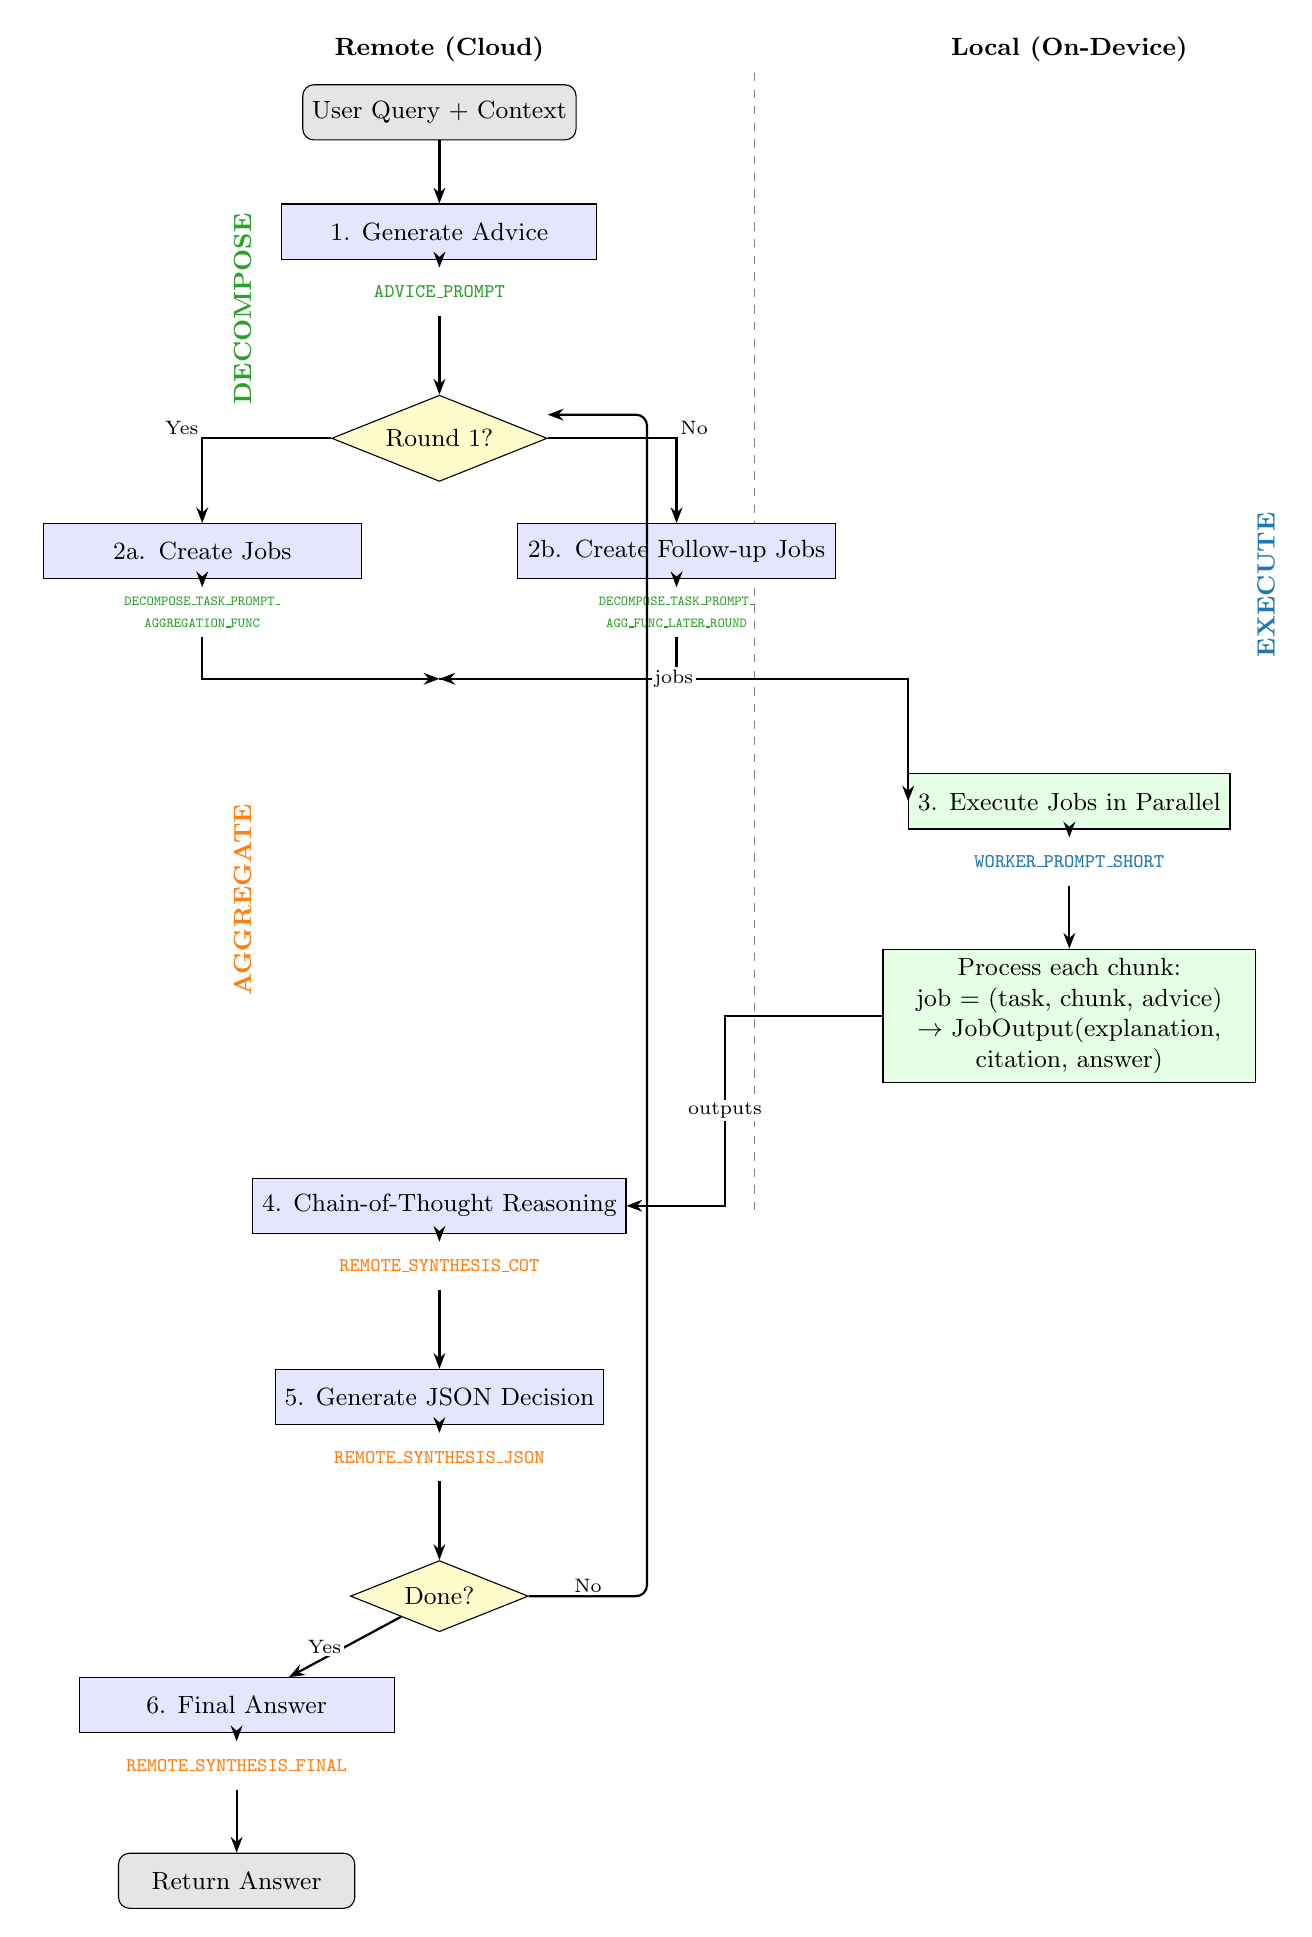
\begin{tikzpicture}[
    node distance=1cm and 2cm,
    >={Stealth[length=2mm]},
    % Node styles
    startstop/.style={rectangle, rounded corners, minimum width=3cm, minimum height=0.7cm, 
                      text centered, draw=black, fill=gray!20, font=\small},
    remote/.style={rectangle, minimum width=4cm, minimum height=0.7cm, 
                   text centered, draw=black, fill=blue!10, font=\small},
    local/.style={rectangle, minimum width=4cm, minimum height=0.7cm, 
                  text centered, draw=black, fill=green!10, font=\small},
    prompt/.style={rectangle, minimum width=3.8cm, minimum height=0.6cm, 
                   text centered, font=\scriptsize\ttfamily},
    decision/.style={diamond, aspect=2.5, minimum width=1.5cm, 
                     text centered, draw=black, fill=yellow!20, font=\small},
    arrow/.style={thick, ->},
    label/.style={font=\scriptsize, fill=white, inner sep=1pt}
]

% Column labels
\node[font=\small\bfseries] at (-4, 0.8) {Remote (Cloud)};
\node[font=\small\bfseries] at (4, 0.8) {Local (On-Device)};

% Vertical divider
\draw[dashed, gray] (0, 0.5) -- (0, -14);

% Start
\node (start) [startstop] at (-4, 0) {User Query + Context};

% DECOMPOSE Module
\node (advice) [remote, below=0.8cm of start] {1. Generate Advice};
\node (advicep) [prompt, decompgreen, below=0.1cm of advice] {ADVICE\_PROMPT};

\node (roundcheck) [decision, below=1cm of advicep] {Round 1?};

\node (decomp1) [remote, below left=0.8cm and 0.3cm of roundcheck, text width=3.8cm, align=center] {2a. Create Jobs};
\node (decomp1p) [prompt, decompgreen, below=0.1cm of decomp1, text width=4.2cm, align=center] {\tiny DECOMPOSE\_TASK\_PROMPT\_\\AGGREGATION\_FUNC};

\node (decompN) [remote, below right=0.8cm and 0.3cm of roundcheck, text width=3.8cm, align=center] {2b. Create Follow-up Jobs};
\node (decompNp) [prompt, decompgreen, below=0.1cm of decompN, text width=4.2cm, align=center] {\tiny DECOMPOSE\_TASK\_PROMPT\_\\AGG\_FUNC\_LATER\_ROUND};

% Merge point for decompose
\node (decompmerge) [coordinate, below=2.5cm of roundcheck] {};

% EXECUTE Module  
\node (execute) [local, below=1.2cm of decompmerge, xshift=8cm] {3. Execute Jobs in Parallel};
\node (executep) [prompt, execblue, below=0.1cm of execute] {WORKER\_PROMPT\_SHORT};

% Worker details
\node (workers) [local, below=0.8cm of executep, minimum height=1.2cm, text width=4.5cm, align=center] 
    {Process each chunk:\\job = (task, chunk, advice)\\$\rightarrow$ JobOutput(explanation,\\citation, answer)};

% AGGREGATE Module
\node (synthcot) [remote, below=1.2cm of workers, xshift=-8cm] {4. Chain-of-Thought Reasoning};
\node (synthcotp) [prompt, aggorange, below=0.1cm of synthcot] {REMOTE\_SYNTHESIS\_COT};

\node (synthjson) [remote, below=1cm of synthcotp] {5. Generate JSON Decision};
\node (synthjsonp) [prompt, aggorange, below=0.1cm of synthjson] {REMOTE\_SYNTHESIS\_JSON};

\node (decide) [decision, below=1cm of synthjsonp] {Done?};

\node (final) [remote, below left=0.8cm and 0cm of decide] {6. Final Answer};
\node (finalp) [prompt, aggorange, below=0.1cm of final] {REMOTE\_SYNTHESIS\_FINAL};

\node (done) [startstop, below=0.8cm of finalp] {Return Answer};

% Arrows
\draw [arrow] (start) -- (advice);
\draw [arrow] (advice) -- (advicep);
\draw [arrow] (advicep) -- (roundcheck);
\draw [arrow] (roundcheck) -| node[label, above left] {Yes} (decomp1);
\draw [arrow] (roundcheck) -| node[label, above right] {No} (decompN);
\draw [arrow] (decomp1) -- (decomp1p);
\draw [arrow] (decompN) -- (decompNp);
\draw [arrow] (decomp1p.south) |- (decompmerge);
\draw [arrow] (decompNp.south) |- (decompmerge);
\draw [arrow] (decompmerge) -| node[label, pos=0.25] {jobs} (execute.west);
\draw [arrow] (execute) -- (executep);
\draw [arrow] (executep) -- (workers);
\draw [arrow] (workers.west) -- ++(-2,0) |- node[label, pos=0.25] {outputs} (synthcot.east);
\draw [arrow] (synthcot) -- (synthcotp);
\draw [arrow] (synthcotp) -- (synthjson);
\draw [arrow] (synthjson) -- (synthjsonp);
\draw [arrow] (synthjsonp) -- (decide);
\draw [arrow] (decide) -- node[label, left] {Yes} (final);
\draw [arrow] (final) -- (finalp);
\draw [arrow] (finalp) -- (done);

% Loop back arrow - goes to later round prompt
\draw [arrow, rounded corners] (decide.east) -- ++(1.5,0) node[label, above, midway] {No} |- ([yshift=0.3cm]roundcheck.east);

% Module labels on right side
\node[decompgreen, font=\small\bfseries, rotate=90] at (-6.5, -2.5) {DECOMPOSE};
\node[execblue, font=\small\bfseries, rotate=90] at (6.5, -6) {EXECUTE};
\node[aggorange, font=\small\bfseries, rotate=90] at (-6.5, -10) {AGGREGATE};

\end{tikzpicture}
\end{center}

\vspace{1em}
\noindent\textbf{Key:}
\begin{itemize}
  \item \colorbox{blue!10}{Blue boxes}: Remote LLM operations (cloud)
  \item \colorbox{green!10}{Green boxes}: Local LLM operations (on-device)
  \item \textcolor{decompgreen}{\texttt{Green prompts}}: DECOMPOSE module
  \item \textcolor{execblue}{\texttt{Blue prompts}}: EXECUTE module
  \item \textcolor{aggorange}{\texttt{Orange prompts}}: AGGREGATE module
\end{itemize}

%==============================================================================
\section{Prompt-to-Module Mapping}
%==============================================================================

\begin{center}
\small
\begin{tabular}{lll}
\toprule
\textbf{Prompt Name} & \textbf{Module} & \textbf{When Used} \\
\midrule
\texttt{ADVICE\_PROMPT} & \textcolor{decompgreen}{DECOMPOSE} & Initial guidance \\
\texttt{DECOMPOSE\_TASK\_PROMPT\_AGGREGATION\_FUNC} & \textcolor{decompgreen}{DECOMPOSE} & Round 1 \\
\texttt{DECOMPOSE\_TASK\_PROMPT\_AGG\_FUNC\_LATER\_ROUND} & \textcolor{decompgreen}{DECOMPOSE} & Rounds 2+ \\
\midrule
\texttt{WORKER\_PROMPT\_SHORT} & \textcolor{execblue}{EXECUTE} & Local worker execution \\
\midrule
\texttt{REMOTE\_SYNTHESIS\_COT} & \textcolor{aggorange}{AGGREGATE} & Chain-of-thought \\
\texttt{REMOTE\_SYNTHESIS\_JSON} & \textcolor{aggorange}{AGGREGATE} & Decision output \\
\texttt{REMOTE\_SYNTHESIS\_FINAL} & \textcolor{aggorange}{AGGREGATE} & Force final answer \\
\bottomrule
\end{tabular}
\end{center}

\noindent\textbf{Note:} Retrieval variants (\texttt{DECOMPOSE\_RETRIEVAL\_TASK\_PROMPT\_*}) exist but share the same structure with BM25 instructions embedded.

%==============================================================================
\section{Prompt Definitions}
%==============================================================================

%------------------------------------------------------------------------------
\vspace{1em}
\noindent\textbf{\textcolor{decompgreen}{ADVICE\_PROMPT}} --- Generates advice for workers on what information to extract.

\begin{promptbox}{ADVICE\_PROMPT}
\begin{lstlisting}
We need to answer the following question based on {metadata}.: 

## Question
{query}

---

Please provide succinct advice on the critical information we need to extract 
from the {metadata} to answer this question. 

Also consider the following constraints:
- In your response do NOT use numbered lists.
- Do NOT structure your response as a sequence of steps.
\end{lstlisting}
\end{promptbox}

%------------------------------------------------------------------------------
\vspace{1em}
\noindent\textbf{\textcolor{decompgreen}{DECOMPOSE\_TASK\_PROMPT\_AGGREGATION\_FUNC}} --- Main decomposition prompt for Round 1, requiring two Python functions: \texttt{prepare\_jobs()} and \texttt{transform\_outputs()}.

\begin{promptbox}{DECOMPOSE\_TASK\_PROMPT\_AGGREGATION\_FUNC}
\begin{lstlisting}
# Decomposition Round #{step_number}

You (the supervisor) cannot directly read the document(s). Instead, you can 
assign small, isolated tasks to a less capable worker model that sees only 
a single chunk of text at a time.

## Your Job: Write Two Python Functions

### FUNCTION #1: `prepare_jobs(context, prev_job_manifests, prev_job_outputs)`
- Break the document(s) into chunks
- Each job must be **atomic** and require only information from the **single chunk**
- If you need to repeat the same task on multiple chunks, **re-use** the same `task_id`
- Limit yourself to **up to {num_tasks_per_round} tasks** total

## BM25 Retrieval Instructions
- For each subtask you create, create keywords for retrieving relevant chunks. 
  Extract precise keyword search queries that are **directly derived** from 
  the user's question and the subtask.
- Assign high weights to the most essential terms (e.g. terms, dates, numerical 
  values) to maximize retrieval accuracy.
- Choose a higher value for `k` (15) if you are unconfident about your keywords.

### FUNCTION #2: `transform_outputs(jobs) -> str`
- Accepts the worker outputs for the tasks you assigned
- Apply any **filtering logic** (e.g., drop irrelevant or empty results)
- **Aggregate outputs** by `task_id` and `chunk_id`
- Return one **aggregated string** suitable for further supervisor inspection

## Important Reminders:
- **DO NOT** assign tasks that require reading multiple chunks
- Keep tasks **chunk-local and atomic**
- **You** (the supervisor) are responsible for aggregating outputs
\end{lstlisting}
\end{promptbox}

%------------------------------------------------------------------------------
\vspace{1em}
\noindent\textbf{\textcolor{decompgreen}{DECOMPOSE\_TASK\_PROMPT\_AGG\_FUNC\_LATER\_ROUND}} --- Decomposition prompt for Rounds 2+, with access to previous job outputs.

\begin{promptbox}{DECOMPOSE\_TASK\_PROMPT\_AGG\_FUNC\_LATER\_ROUND}
\begin{lstlisting}
# Decomposition Round #{step_number}

You do not have access to the raw document(s), but instead can assign tasks 
to small and less capable language models that can read the document(s).
Note that the document(s) can be very long, so each task should be performed 
only over a small chunk of text. 

# Your job is to write two Python functions:

Function #1 (prepare_jobs): will output formatted tasks for a small language model.
-> Make sure that NONE of the tasks require multiple steps. Each task should be atomic! 
-> Consider using nested for-loops to apply a set of tasks to a set of chunks.
-> The same `task_id` should be applied to multiple chunks. 
-> Use the conversational history to inform what chunking strategy has been applied.
-> You are provided access to the outputs of the previous jobs (see prev_job_outputs). 
-> If helpful, you can reason over the prev_job_outputs vs. the original context.
-> If tasks should be done sequentially, wait for the next round.

## BM25 Retrieval Instructions
- For each subtask you create, create keywords for retrieving relevant chunks. 
  Extract precise keyword search queries that are **directly derived** from 
  the user's question and the subtask.
- Assign high weights to the most essential terms (e.g. terms, dates, numerical 
  values) to maximize retrieval accuracy.
- Choose a higher value for `k` (15) if you are unconfident about your keywords.

Function #2 (transform_outputs): aggregate outputs for supervisor review.
-> Filter jobs based on output (write a custom filter function). 
-> Aggregate the jobs based on the task_id and chunk_id.

## Using Previous Round Information
Our conversation history includes information about previous rounds of jobs 
and their outputs. Use this information to inform your new jobs:
- Based on the Job outputs above, subselect `chunk_id`s that require further 
  reasoning and are relevant to the question
- Reformat tasks that are not yet complete.
- Make your `advice` more concrete. 
\end{lstlisting}
\end{promptbox}

%------------------------------------------------------------------------------
\vspace{1em}
\noindent\textbf{\textcolor{execblue}{WORKER\_PROMPT\_SHORT}} --- Local worker prompt using Pydantic model specification.

\begin{promptbox}{WORKER\_PROMPT\_SHORT}
\begin{lstlisting}
Here is a document excerpt:

{context}

--------------------------------
And here is your task:

{task}

--------------------------------
And here is additional higher-level advice on how to approach the task:

{advice}

--------------------------------

Your response should be a `JobOutput` object:
```python
class JobOutput(BaseModel):
  explanation: str  # A concise statement of your reasoning
  citation: str | None  # A direct snippet supporting your answer
  answer: str | None  # Your answer to the question
```
Your response:
\end{lstlisting}
\end{promptbox}

%------------------------------------------------------------------------------
\vspace{1em}
\noindent\textbf{\textcolor{aggorange}{REMOTE\_SYNTHESIS\_COT}} --- Chain-of-thought synthesis prompt for step-by-step reasoning.

\begin{promptbox}{REMOTE\_SYNTHESIS\_COT}
\begin{lstlisting}
Now synthesize the findings from multiple junior workers (LLMs). 
Your task is to analyze the collected information and think step-by-step 
about whether we can answer the question. Be brief and concise.

## Previous Progress
{scratchpad}

## Inputs
1. Question to answer: {question}
2. Collected Job Outputs (from junior models): {extractions}

## Instructions
Think step-by-step about:
1. What information we have gathered
2. Whether it is sufficient to answer the question
3. If not sufficient, what specific information is missing
4. If sufficient, how we would calculate or derive the answer
5. If there are conflicting answers: Use citations to select the correct one

Be brief and concise. No need for structured output.
\end{lstlisting}
\end{promptbox}

%------------------------------------------------------------------------------
\vspace{1em}
\noindent\textbf{\textcolor{aggorange}{REMOTE\_SYNTHESIS\_JSON}} --- JSON output format specification for synthesis decisions.

\begin{promptbox}{REMOTE\_SYNTHESIS\_JSON}
\begin{lstlisting}
Based on your analysis, return a single JSON object:

{
  "explanation": "",
  "feedback": null,
  "decision": "",
  "answer": null,
  "scratchpad": ""
}

Field Descriptions:
- explanation: A brief statement of your reasoning
- feedback: Specific information to look for, if needed (null if not applicable)
- decision: Either "provide_final_answer" or "request_additional_info"
- answer: The final answer if providing one; null otherwise
- scratchpad: Summary of gathered information for future reference
\end{lstlisting}
\end{promptbox}

%------------------------------------------------------------------------------
\vspace{1em}
\noindent\textbf{\textcolor{aggorange}{REMOTE\_SYNTHESIS\_FINAL}} --- Final answer synthesis prompt (forces a final answer).

\begin{promptbox}{REMOTE\_SYNTHESIS\_FINAL}
\begin{lstlisting}
Now provide the final answer based on all gathered information.

## Previous Progress
{scratchpad}

## Inputs
1. Question to answer: {question}
2. Collected Job Outputs (from junior models): {extractions}

Return a single JSON object:
{
  "explanation": "",
  "feedback": null,
  "decision": "",
  "answer": null,
  "scratchpad": ""
}

Field Descriptions:
- explanation: Brief statement of your reasoning
- feedback: Any specific information lacking (NO CODE). Use null if not needed
- decision: must be "provide_final_answer"
- answer: Final answer
- scratchpad: Summary of gathered information
\end{lstlisting}
\end{promptbox}

\end{document}
